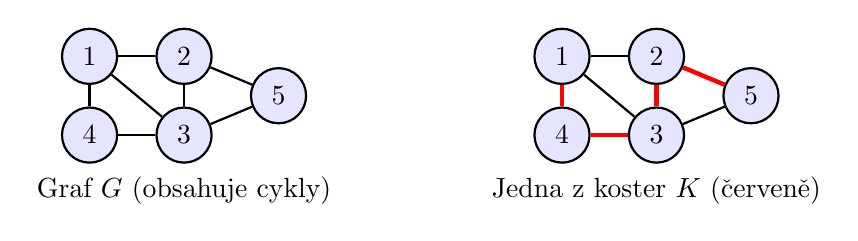
\begin{tikzpicture}[
  vnode/.style={circle, draw, minimum size=7mm, inner sep=0pt, fill=blue!10},
  thick
]
  % Původní graf G
  \begin{scope}[shift={(-3,0)}]
    \node[vnode] (1) at (0, 1) {1};
    \node[vnode] (2) at (1.2, 1) {2};
    \node[vnode] (3) at (1.2, 0) {3};
    \node[vnode] (4) at (0, 0) {4};
    \node[vnode] (5) at (2.4, 0.5) {5};
    
    \draw (1) -- (2); \draw (2) -- (3); \draw (3) -- (4); \draw (4) -- (1);
    \draw (1) -- (3); \draw (2) -- (5); \draw (3) -- (5);
    \node at (1.2, -0.7) {Graf $G$ (obsahuje cykly)};
  \end{scope}

  % Kostra K
  \begin{scope}[shift={(3,0)}]
    \node[vnode] (1') at (0, 1) {1};
    \node[vnode] (2') at (1.2, 1) {2};
    \node[vnode] (3') at (1.2, 0) {3};
    \node[vnode] (4') at (0, 0) {4};
    \node[vnode] (5') at (2.4, 0.5) {5};
    
    % Další hrany (nepatřící do kostry)
    \draw (1') -- (2');
    \draw (1') -- (3');
    \draw (3') -- (5');
    % Kostra (červeně a zvýrazněno)
    \draw[red, ultra thick] (1') -- (4');
    \draw[red, ultra thick] (4') -- (3');
    \draw[red, ultra thick] (3') -- (2');
    \draw[red, ultra thick] (2') -- (5');
    \node at (1.2, -0.7) {Jedna z koster $K$ (červeně)};
  \end{scope}
\end{tikzpicture}
\par\medskip
\textit{Obrázek 1.2: Ukázka souvislého grafu $G$ a jedné z jeho možných koster $K$.}